
\chapter{Documentación de HARDroid}
\label{index:har-index}\label{index:hardroid}\label{index:human-activity-recognition-for-android}

\section{Acerca de HARDroid}
\label{index:bienvenido-a-la-documentacion-de-hardroid}
Este proyecto es un servicio de reconocimiento de actividades humanas
para Android. Utiliza dos componentes, una librería y una aplicación de servicio instalable por \abbr{APK}.

El estado y avances del proyecto está disponible en el repositorio GitHub \cite{GimenezYegros2016c} y también verificar la documentación \emph{Java} en \cite{GimenezYegros2016d} para más detalles sobre el funcionamiento de la \abbr{API}.


\subsection{Autores}
\label{index:autores}\begin{itemize}
\item {} 
    Alberto G. (\url{https://github.com/agimenezpy})

\item {} 
    Santiago Y. (\url{https://github.com/syegros})

\end{itemize}
\phantomsection\label{index:har-content}

\subsection{¿Qué es HARDroid?}
\label{intro:har-intro}\label{intro::doc}\label{intro:que-es-hardroid}

\subsubsection{HARDroid}
\label{intro:hardroid}
\abbr{HARDroid} es el proyecto \emph{Open Source} cuyo objetivo es tener una implementación abierta de un servicio de
reconocimiento de actividades humanas utilizando sensores del teléfono.

Este proyecto implementa el desacomplamiento por medio de una librería que expone una \abbr{API} y una aplicación de servicio en forma de \abbr{APK} independiente que provee las
funcionalidades.

La idea se basa en los productos similares de las corporaciones Google y Sony, que permiten reconocer actividades por medio de \emph{Google Play Services} y \emph{Sony LifeLog}.

\subsubsection{Google Play Services}
\label{intro:har-google-play-services}\label{intro:google-play-services}
La corporación Google publica como producto a Google Play Services \cite{Google2016ps} donde proporciona dentro de una \abbr{APK} la implementación de diversas funcionalides, y donde los desarrolladores de aplicaciones
\emph{Android} pueden integrarse (a través de una \abbr{API} \cite{Google2016l}) en las siguientes dimensiones:
\begin{quote}
\begin{description}
\item[{Location \& Context}] \leavevmode
Provee funcionalidades para mejorar la precisión y calidad de la ubicación GPS del celular basado en sensores.
Además, la función \emph{contexto} provee la capacidad de reconocer las actividades físicas

\item[{Ads}] \leavevmode
Provee funcionalidades para ofrecer publicidad in la aplicación

\item[{Games}] \leavevmode
Provee funcionalidades para Gamificar la aplicación

\item[{Cloud Messaging}] \leavevmode
Provee funcionalidades para mensajería a travéz de Internet.

\end{description}

\end{quote}

\subsubsection{Sony LifeLog}
\label{intro:sony-lifelog}\label{intro:har-life-log}
La corporación Sony publica un producto llevar un registro de las actividades diarias personales por medio de sensores
en el celular o utilizando relojes \emph{smartwatch} y pulseras. Con el fin de mejorar la experiencia del usuario proveen una aplicación de registro diario con un reconocedor de actividades incorporado.
\begin{table}[!h]
\begin{tabular}{lll}
\textsf{\relax 
Inicio LifeLog
} & \textsf{\relax 
Configuración
} & \textsf{\relax 
Acerca del Reconocedor
}\\
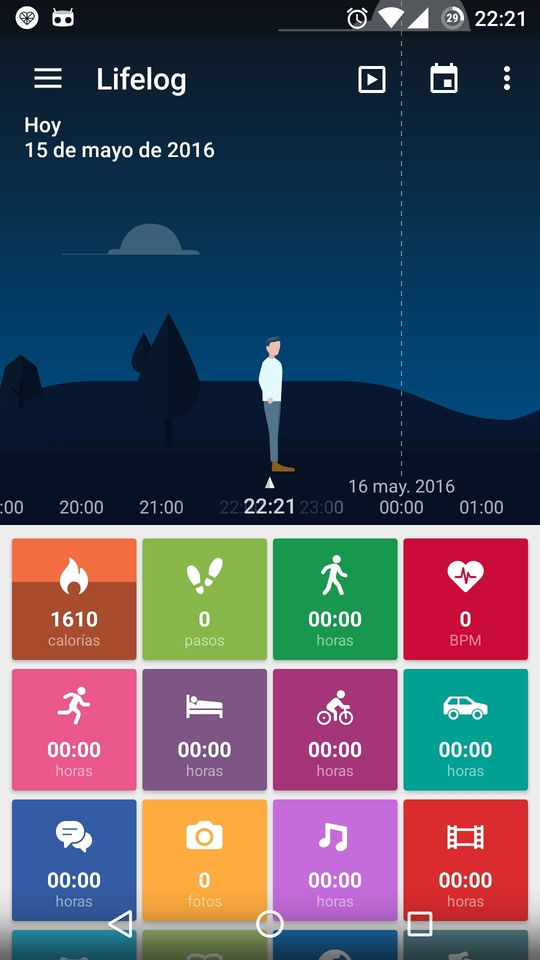
\includegraphics[width=0.33\textwidth]{anexos/graphics/lf_start.jpg}
 & 
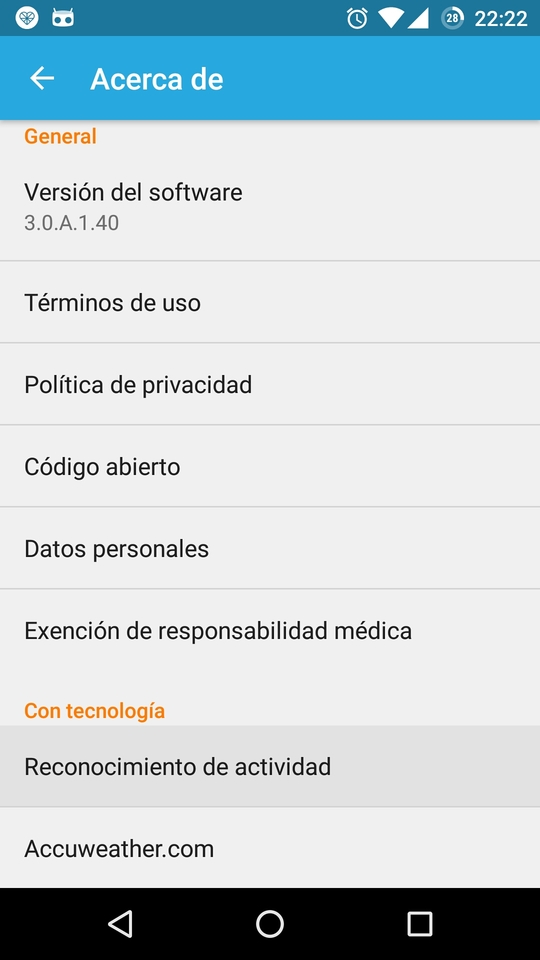
\includegraphics[width=0.33\textwidth]{anexos/graphics/lf_conf.jpg}
 & 
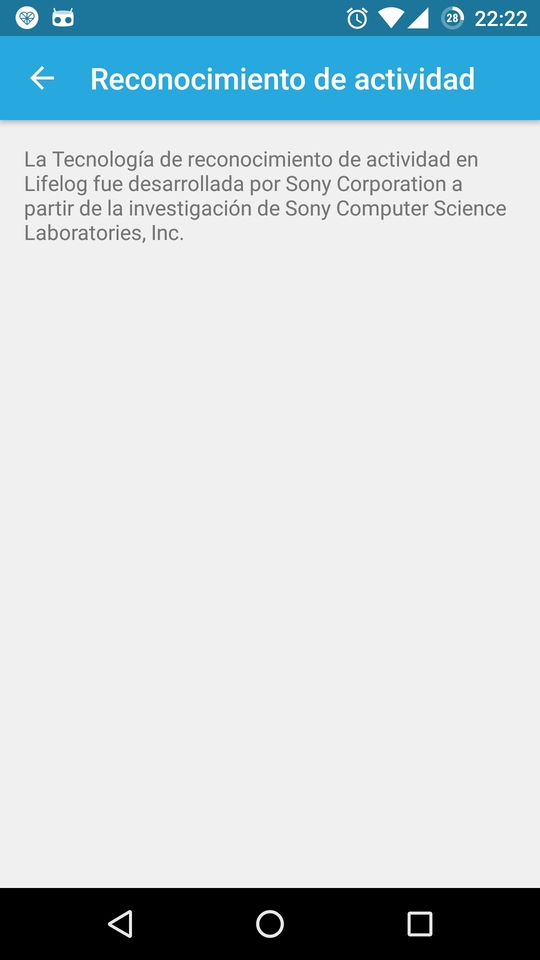
\includegraphics[width=0.33\textwidth]{anexos/graphics/lf_actrec.jpg}
\\
\end{tabular}
\end{table}

\section{Guía de Utilización}
\label{first:har-first}\label{first::doc}\label{first:primeros-pasos}

\subsubsection{Instalar las Aplicaciones}
\label{first:instalar-las-aplicaciones}
El proyecto se compone de dos aplicaciones \emph{\abbr{Android}} que se interaccionan por medio de \abbr{IPC} \emph{BINDER} de manera a
independizar las funciones de encuesta y de servicio de reconocimiento.

\begin{figure}[!h]
\centering
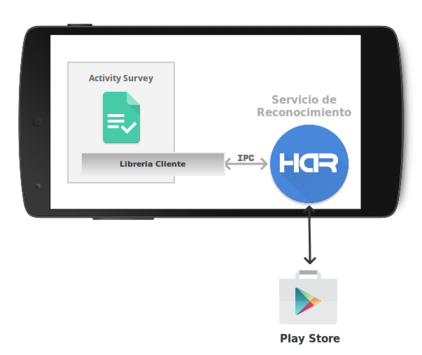
\includegraphics[width=0.7\textwidth]{anexos/graphics/archi_ipc.png}
\end{figure}

Para poder contribuir con la recolección de datos se siguen los siguientes pasos de instalación.

\paragraph{Instalar la Encuesta}
\label{first:instalar-la-encuesta}\label{first:har-survey}
Para instalar la aplicación \emph{Activity Survey} de encuesta accede a este URL \url{https://goo.gl/JHNL1B} o por medio de la siguiente 
imagen:
\begin{figure}[!h]
   \centering
   
\includegraphics{anexos/graphics/qr_url.jpg}
\caption{Acceso al instalador \emph{Activity Survey}}\label{first:id1}\end{figure}

Se debe descargar la aplicación desde el
\emph{Google Play Store} \cite{GimenezYegros2016e} como se muestra en la \figref{first:id2}.
\begin{figure}[!h]
    \centering 
    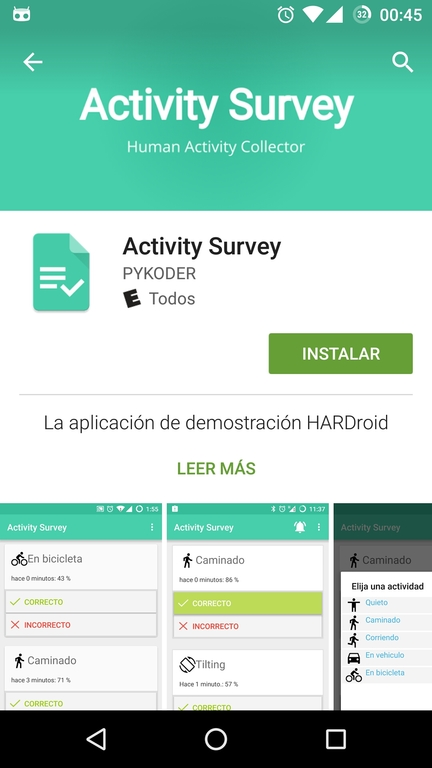
\includegraphics[width=0.4\textwidth]{anexos/graphics/inst_app5.jpg}
\caption{Instalador desde Google Play}\label{first:id2}\end{figure}

En caso de requerir registrarse como \emph{beta tester} proceder a acceder con una cuenta de Google en el enlace \url{https://goo.gl/GjmMl3} y seguir los pasos de la \tabref{tab:betatest}.

\begin{table}[!h]
\begin{tabular}{lll}
\textsf{\relax 
Ingresar el URL
} & \textsf{\relax 
Logearse a Google
} & \textsf{\relax 
Aceptar ser tester
}\\
    {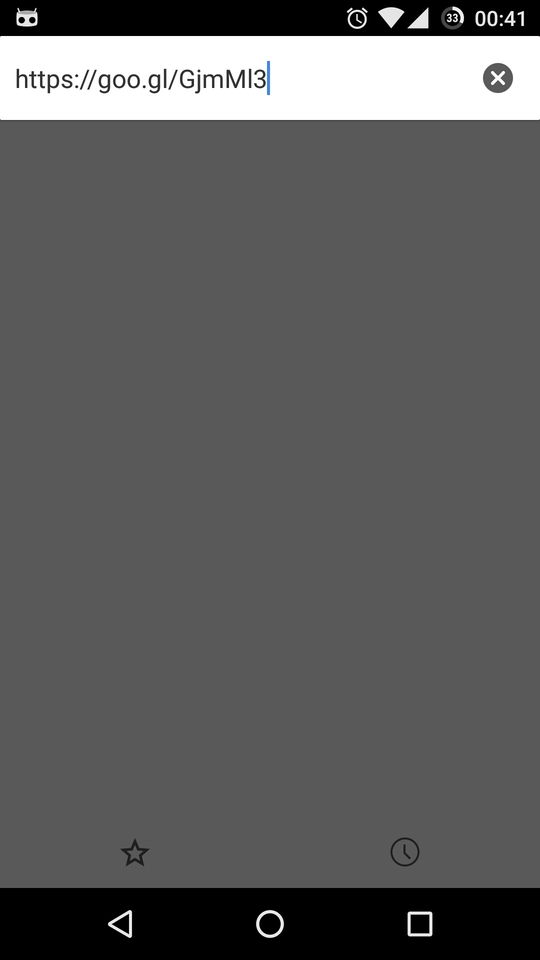
\includegraphics[width=0.33\textwidth]{anexos/graphics/inst_app.jpg}}
 & 
    {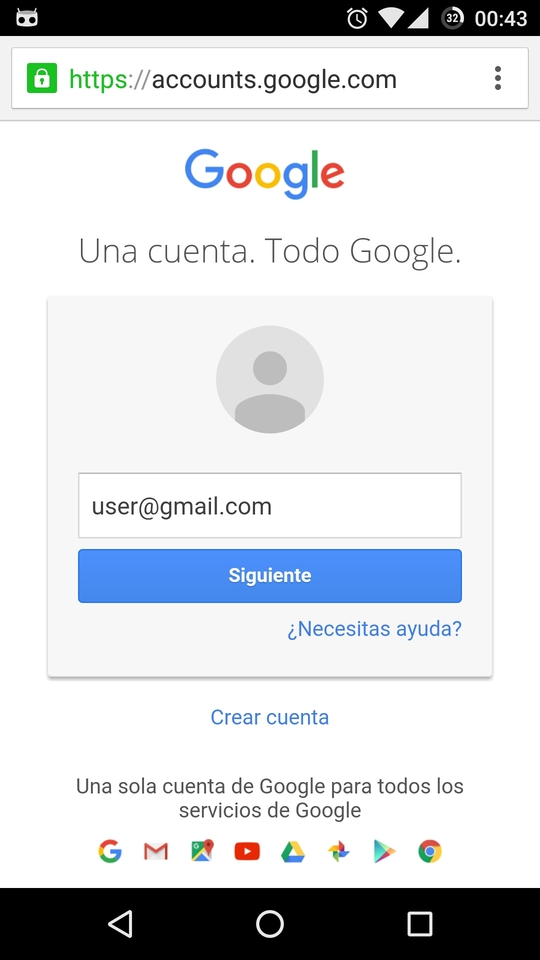
\includegraphics[width=0.33\textwidth]{anexos/graphics/inst_app2.jpg}}
 & 
    {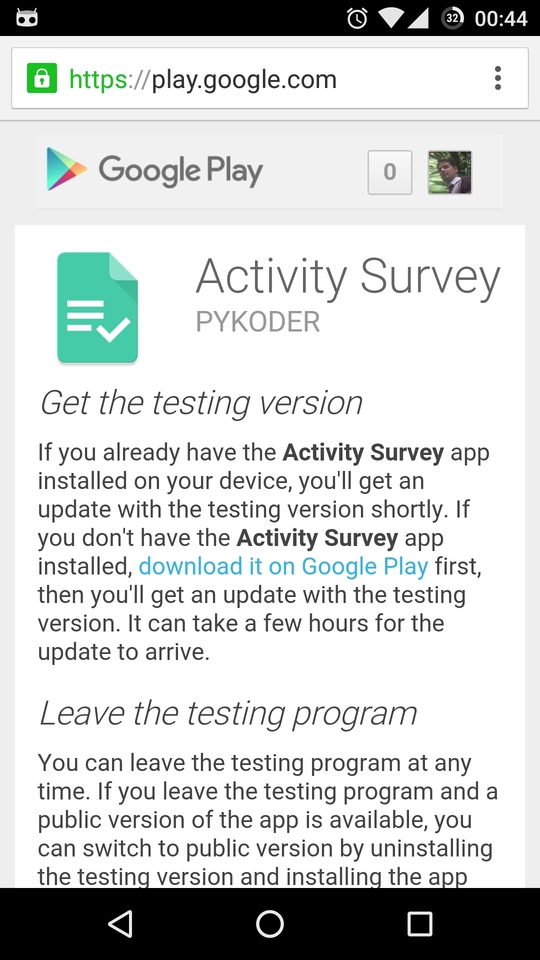
\includegraphics[width=0.33\textwidth]{anexos/graphics/inst_app4.jpg}}
\\
\end{tabular}
\caption{Pasos de registro a \emph{Beta Test}}\label{tab:betatest}
\end{table}


Para finalizar se debe configurar la aplicación siguiendo los pasos en \hyperref[config:har-config]{Configurar Activity Survey}.


\paragraph{Instalar el Reconocedor}
\label{first:instalar-el-reconocedor}
Luego de instalar y configurar la aplicación de encuesta \emph{Activity Survey} (vease {\hyperref[config:har-config]{Configurar Activity Survey}),
al intentar utilizar la aplicación necesitara instalar desde el \emph{Google Play Store} el servicio reconocedor \emph{HARDroid} según la \tabref{tab:hardroid}.

\begin{table}[h]
\begin{tabular}{ll}
\textsf{\relax 
Sugerencia para HARDroid
} & \textsf{\relax 
Instalar del Play Store
}\\
    {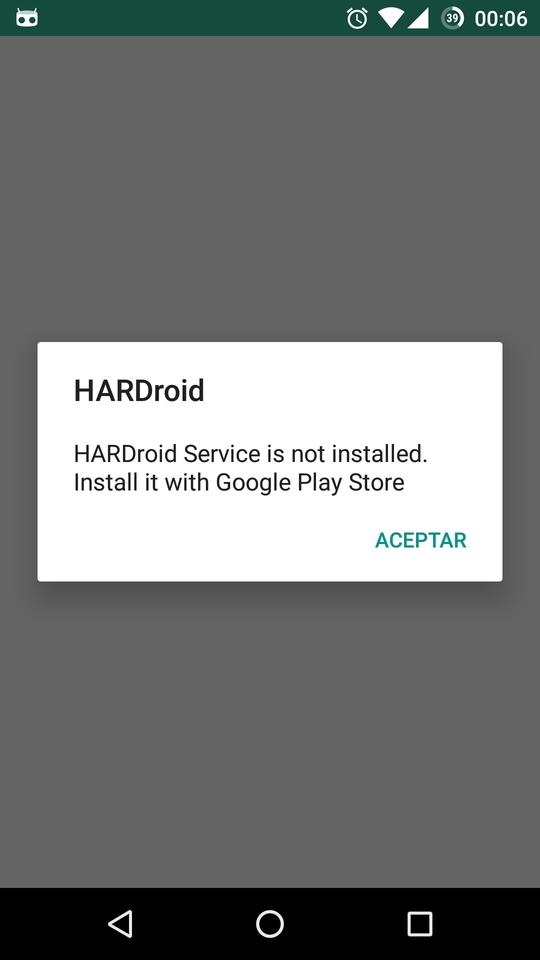
\includegraphics[width=0.33\textwidth]{anexos/graphics/install_service.jpg}}
 & 
    {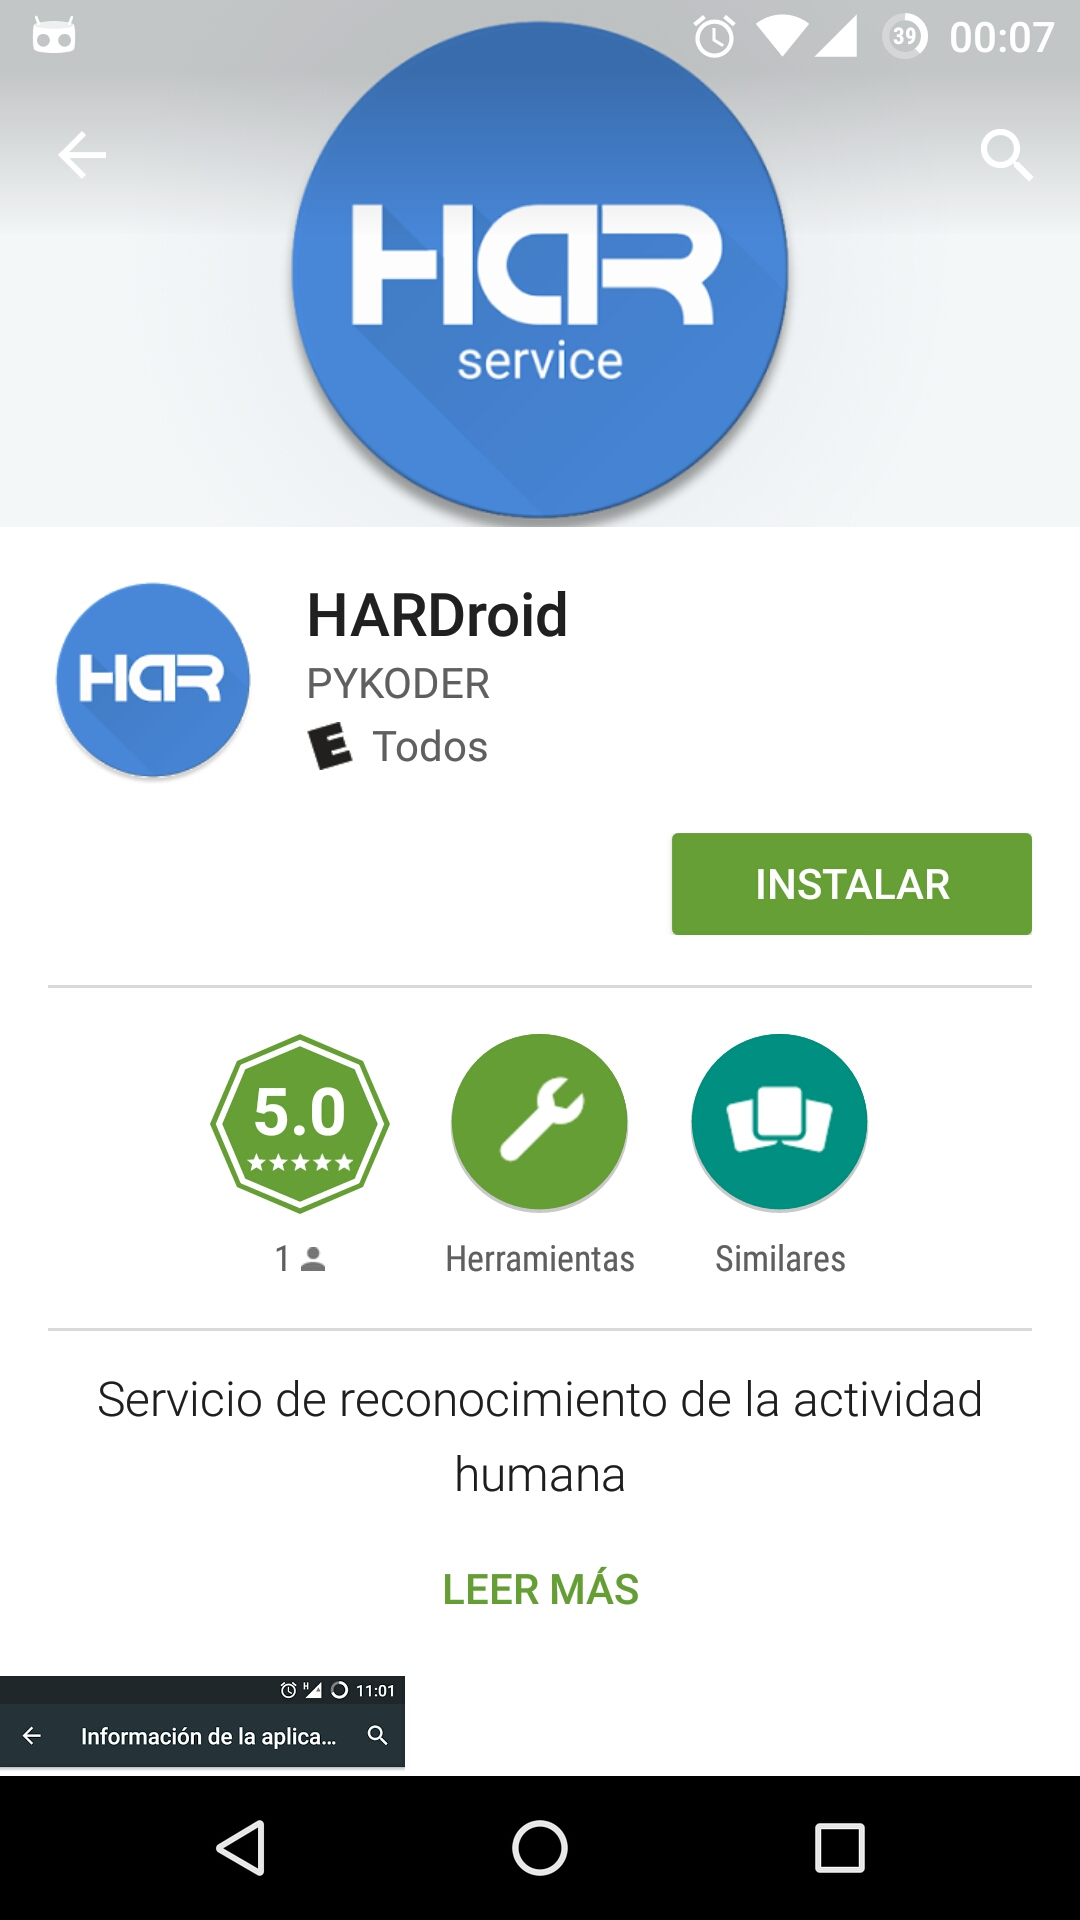
\includegraphics[width=0.33\textwidth]{anexos/graphics/inst_servplay.jpg}}
\\
\end{tabular}
    \caption{Pasos para instalar HARDroid}\label{tab:hardroid}
\end{table}

\subsection{Configurar \emph{Activity Survey}}
\label{config:configurar-activity-survey}\label{config:har-config}\label{config::doc}

\subsubsection{Iniciar la encuesta}
\label{config:iniciar-la-encuesta}
Una vez instalada la aplicación de encuesta se debe configurar los datos mínimos para iniciar la contribución de la recolección. Iniciar la aplicación como en la \figref{config:id1}.
\begin{figure}[!h]
\centering
    {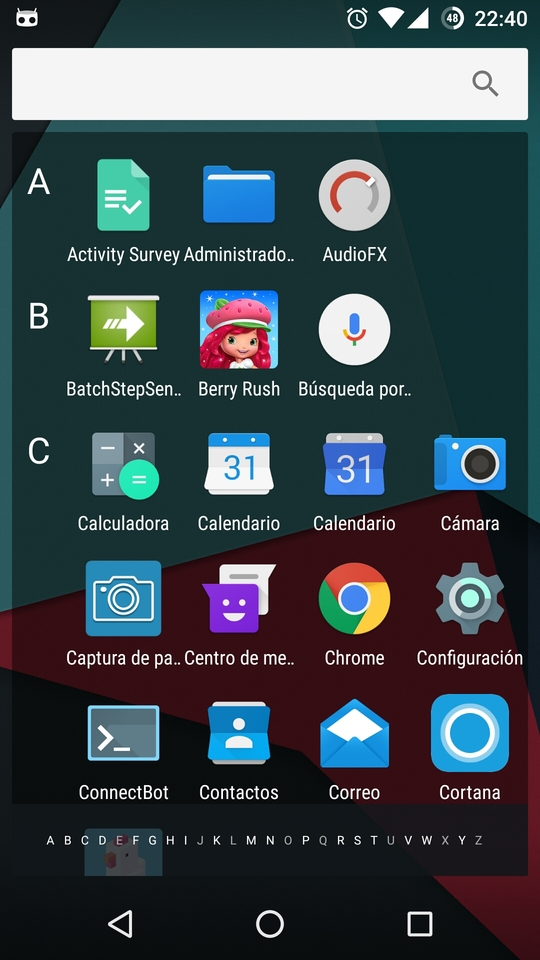
\includegraphics[width=0.4\textwidth]{anexos/graphics/app_inst.jpg}}
\caption{\emph{Activity Survey} instalada}\label{config:id1}\end{figure}

Luego se aceptan las instrucciones y concede los permisos necesarios como en la \tabref{config:iniapp}.

\begin{table}[!h]
\begin{tabular}{lll}
\textsf{\relax 
Iniciar la Encuesta
} & \textsf{\relax 
Aceptar y configurar
} & \textsf{\relax 
Dar permisos
}\\
    {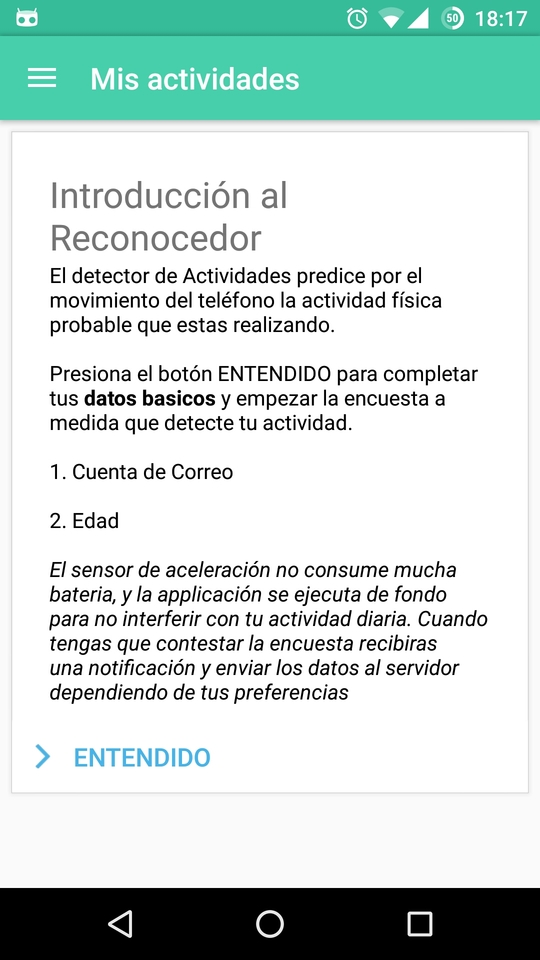
\includegraphics[width=0.33\textwidth]{anexos/graphics/app_start.jpg}}
 & 
    {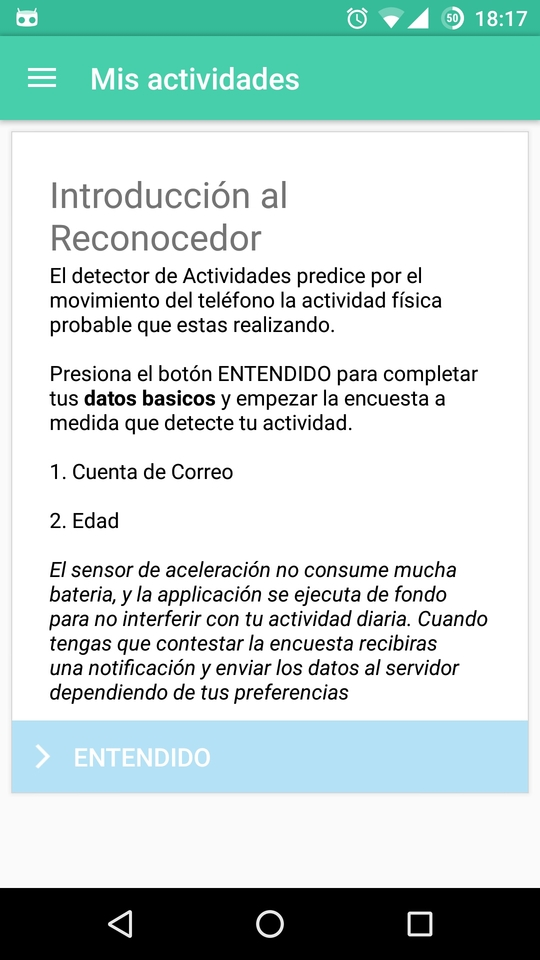
\includegraphics[width=0.33\textwidth]{anexos/graphics/app_start2.jpg}}
 & 
    {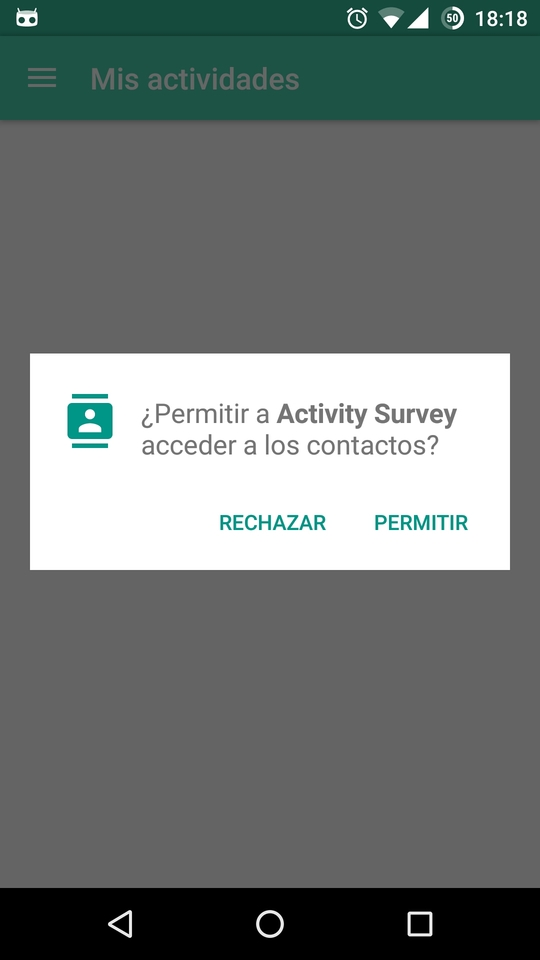
\includegraphics[width=0.33\textwidth]{anexos/graphics/app_perm.jpg}}
\\
\end{tabular}
    \caption{Pasos iniciales para la aplicación de encuesta}\label{config:iniapp}
\end{table}

\subsubsection{Ingresar correo y edad}
\label{config:ingresa-tu-correo-y-edad}
Para poder identificar las contribuciones se requiere de datos mínimos para la encuesta como en la \figref{config:id2}.
\begin{figure}[!h]
\centering
    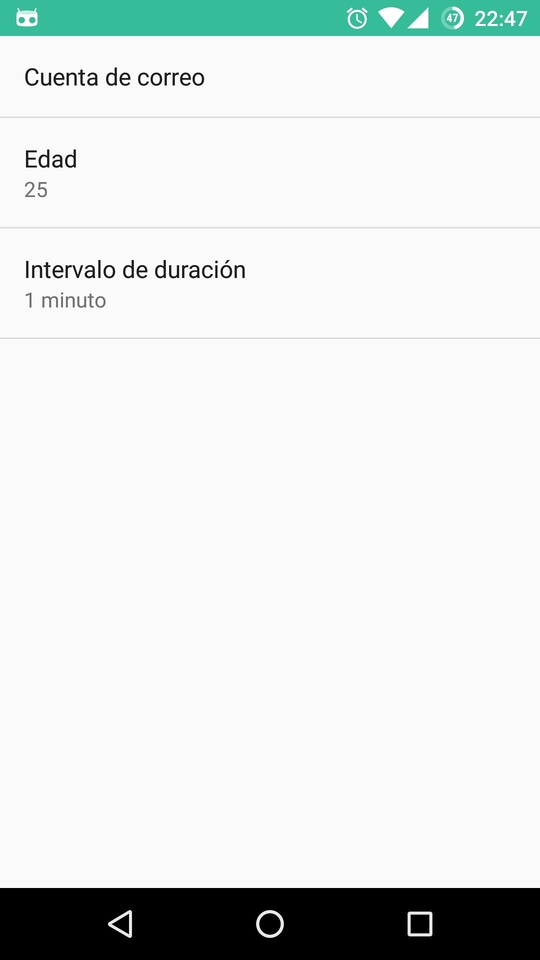
\includegraphics[width=0.4\textwidth]{anexos/graphics/app_conf.jpg}
\caption{Iniciar la configuración}\label{config:id2}\end{figure}

Configurar los datos requeridos como en la \tabref{config:emedad}.
\begin{table}[!h]
\begin{tabular}{lll}
\textsf{\relax 
Ingresa tu correo
} & \textsf{\relax 
Ingresa tu edad
} & \textsf{\relax 
Ingresa el intervalo
}\\
    {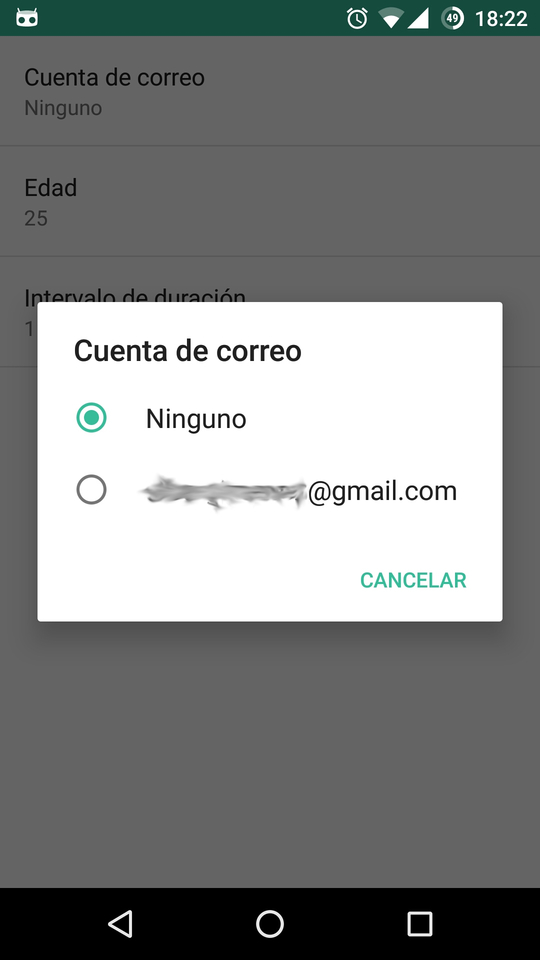
\includegraphics[width=0.33\textwidth]{anexos/graphics/app_email.jpg}}
 & 
    {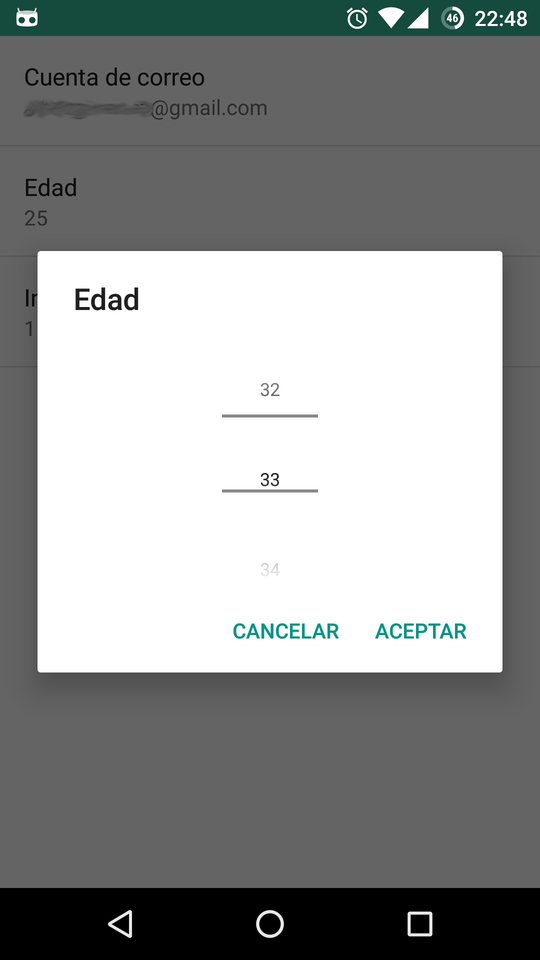
\includegraphics[width=0.33\textwidth]{anexos/graphics/app_age.jpg}}
 & 
    {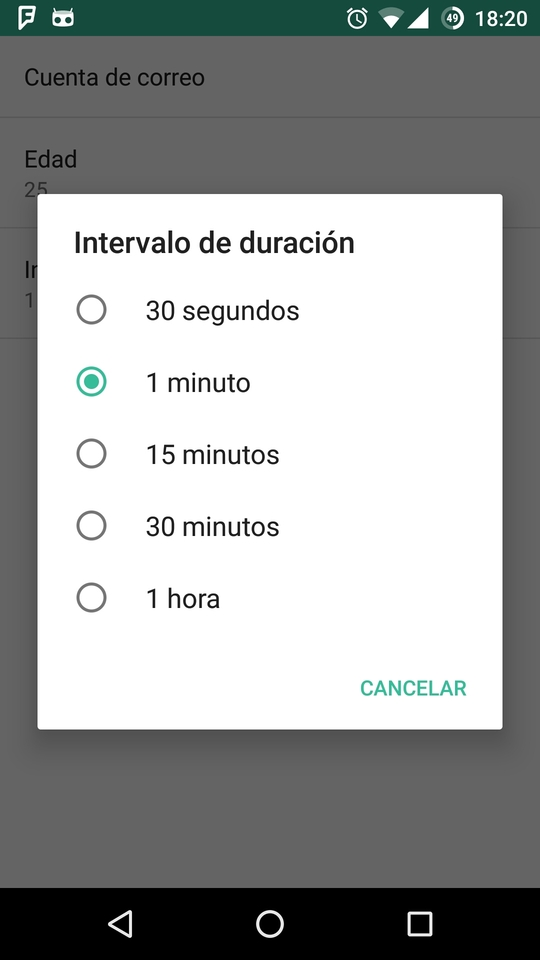
\includegraphics[width=0.33\textwidth]{anexos/graphics/app_int.jpg}}
\\
\end{tabular}
    \caption{Configuración inicial de la aplicación}\label{config:emedad}
\end{table}

El servicio de reconocimiento se activará a cada intervalo que se eliga en la configuración:
\begin{itemize}
\item {} 
1 minuto

\item {} 
15 minutos

\item {} 
30 minutos

\item {} 
1 hora

\end{itemize}

\subsubsection{Servicio de Reconocimiento}
\label{config:servicio-de-reconocimiento-activado}
Una vez configurada la aplicación de encuesta, esta se conectará automáticamente al servicio de reconocimiento instalado una vez que se inicia una sesión de encuesta \figref{config:id3}.
\begin{figure}[!h]
\centering

    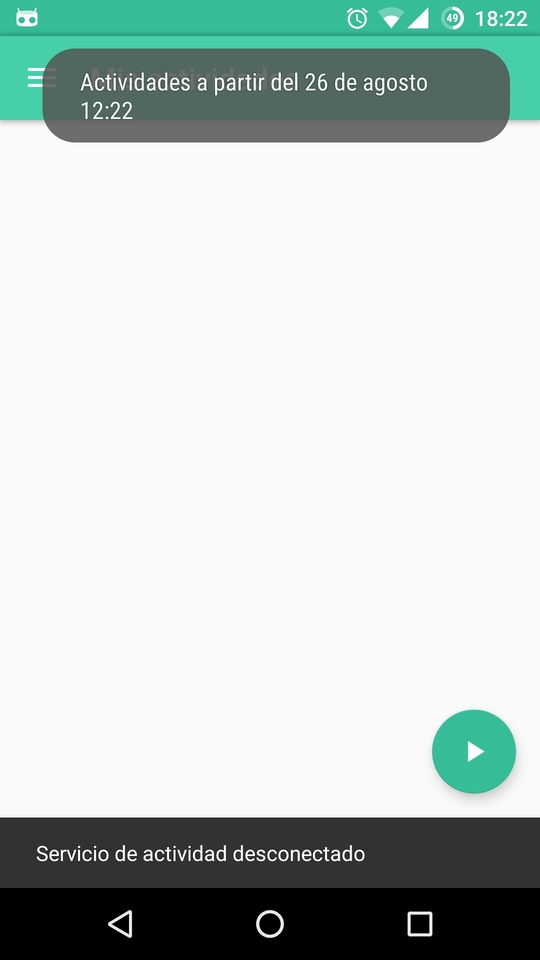
\includegraphics[width=0.4\textwidth]{anexos/graphics/app_started.jpg}
\caption{Servicio de Reconocimiento Iniciado}\label{config:id3}\end{figure}


\subsection{Contribuir con \emph{Activity Survey}}
\label{contrib:har-contrib}\label{contrib::doc}\label{contrib:contribuir-con-activity-survey}

\subsubsection{Ver tus actividades}
\label{contrib:ver-tus-actividades}
Dependiendo del intervalo de reconocimiento la aplicación de encuesta desplegará las últimas actividades recientes
reconocidas en orden descendente como en la \tabref{contrib:actrec}.

\begin{table}[!h]
\begin{tabular}{ll}
\textsf{\relax 
Actividades recientes
} & \textsf{\relax 
Mas actividades
}\\
    {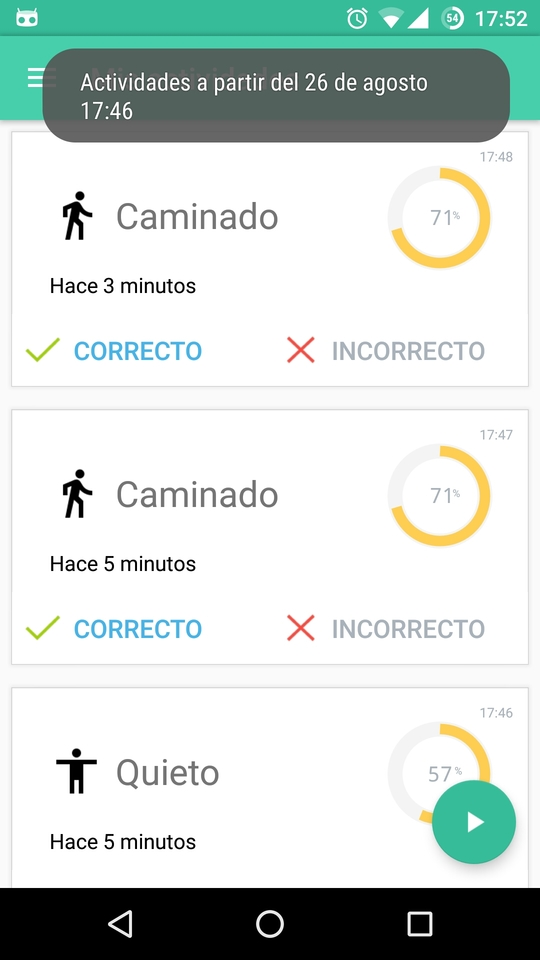
\includegraphics[width=0.33\textwidth]{anexos/graphics/activities_toast.jpg}}
 & 
    {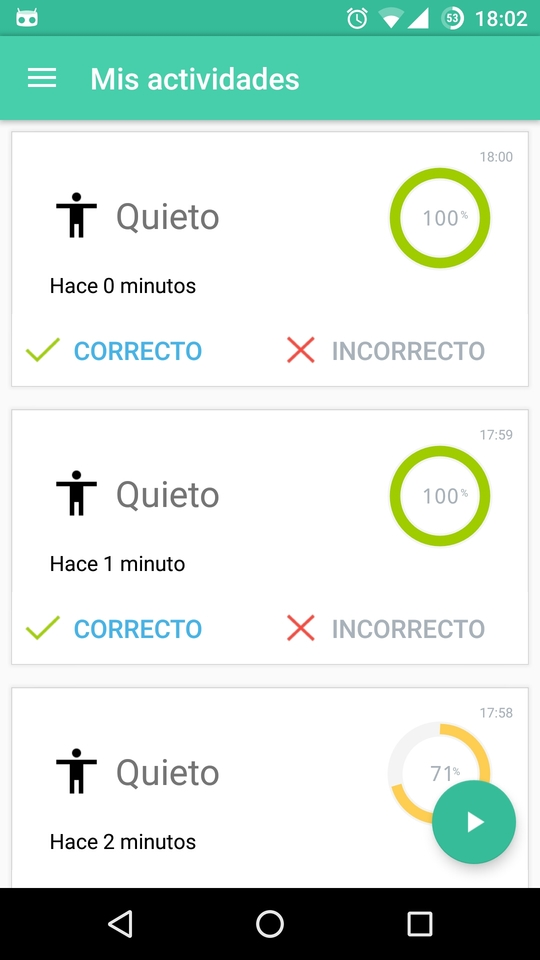
\includegraphics[width=0.33\textwidth]{anexos/graphics/activities.jpg}}
\\
\end{tabular}
    \caption{Despliegue de actividades recientes}\label{contrib:actrec}
\end{table}

Además se reciben notificaciones periodicas a medida que se reconozca una actividad mientras la sesión esté iniciada \tabref{contrib:actnot}.

\begin{table}[!h]
\begin{tabular}{ll}
\textsf{\relax 
Notificación Recibida
} & \textsf{\relax 
Detalle de actividad
}\\
    {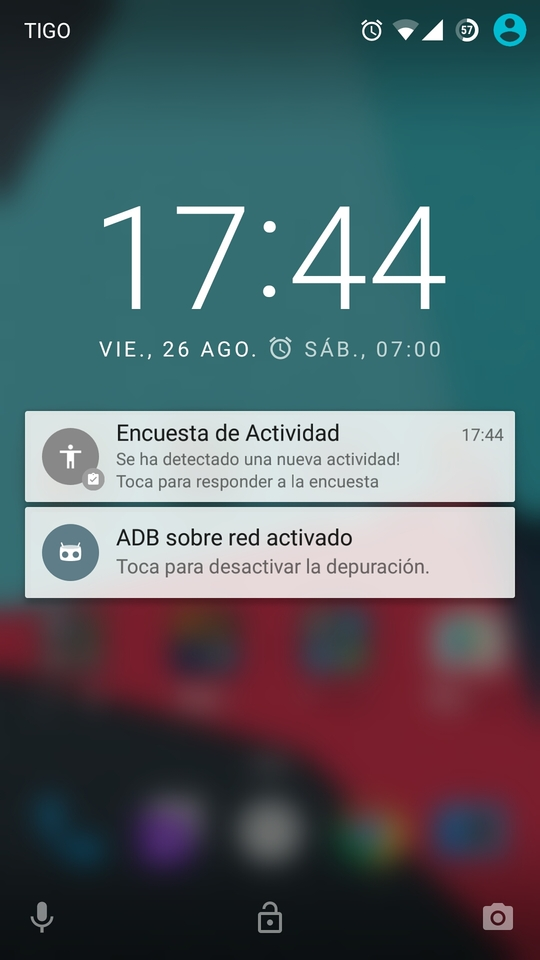
\includegraphics[width=0.33\textwidth]{anexos/graphics/scr_notification.jpg}}
 & 
    {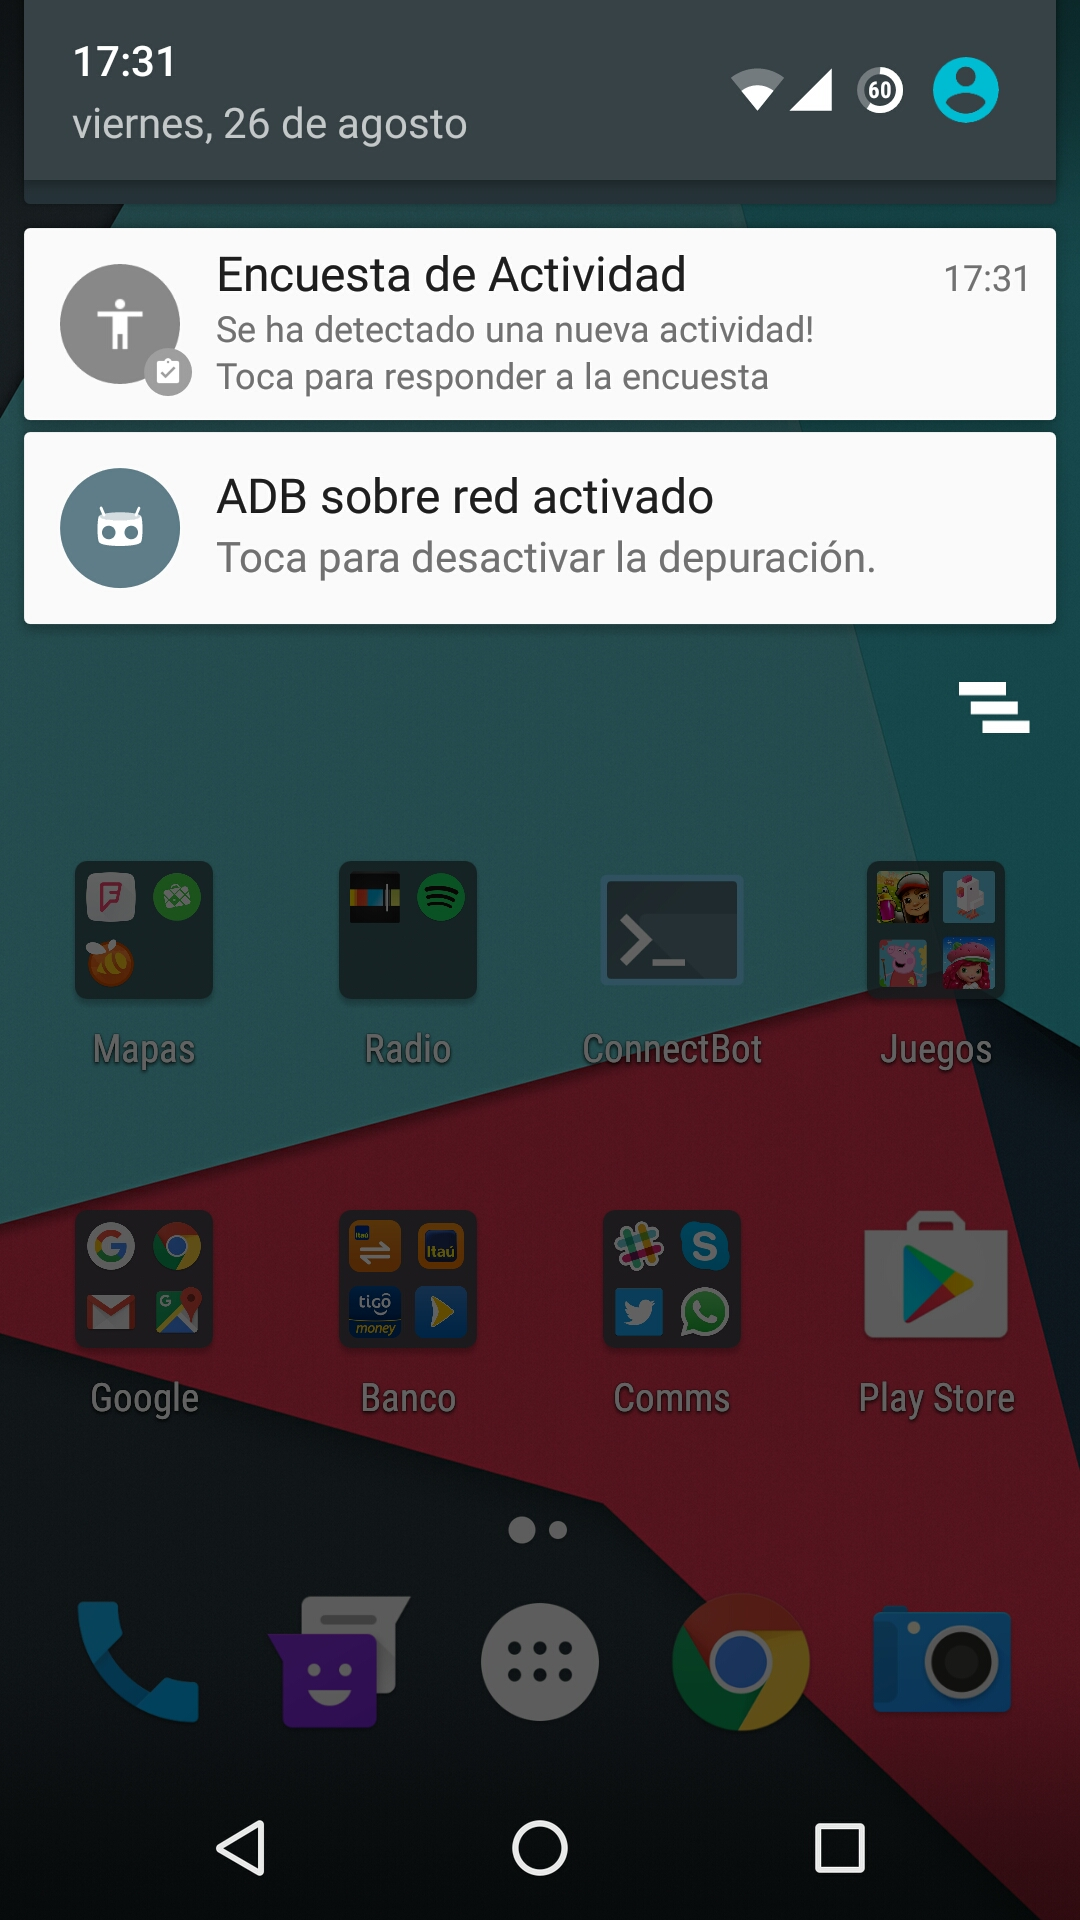
\includegraphics[width=0.33\textwidth]{anexos/graphics/bar_notification2.jpg}}
\\
\end{tabular}
    \caption{Notificaciones de actividades reconocidas}\label{contrib:actnot}
\end{table}

\pagebreak

\subsubsection{Actividades Conocidas}
\label{contrib:actividades-conocidas}
Las actividades reconocidas por el servicio son:
\begin{quote}
\begin{description}
\item[{Quieto}] \leavevmode
El servicio detectó que el teléfono móvil está quieto.


\includegraphics{anexos/graphics/still.png}

\item[{Caminando}] \leavevmode
El servicio detectó que el teléfono móvil está en movimiento lento  
    

\includegraphics{anexos/graphics/walk.png}

\item[{Correr}] \leavevmode
El servicio detectó que el teléfono móvil está en movimiento apresurado.


\includegraphics{anexos/graphics/run.png}

\item[{En vehiculo}] \leavevmode
El servicio detectó que el teléfono móvil está en movimiento dentro de un vehiculo.


\includegraphics{anexos/graphics/car.png}

\item[{En bicicleta}] \leavevmode
El servicio detectó que el teléfono móvil está en movimiento sobre una bicicleta.


\includegraphics{anexos/graphics/bike.png}

\item[{Tilting}] \leavevmode
El servicio detectó que el teléfono móvil está girando.


\includegraphics{anexos/graphics/tilt.png}

\item[{Desconocido}] \leavevmode
El servicio no pudo detectar la actividad.


\includegraphics{anexos/graphics/unk.png}

\end{description}
\end{quote}

\subsubsection{Responder a la Encuesta}
\label{contrib:responder-a-la-encuesta}
Para responder a la encuesta se tienen las siguientes opciones como \tabref{contrib:actres}.
\begin{quote}
\begin{description}
\item[{Actividad Correcta}] \leavevmode
El servicio detecto correctamente la actividad física, marcarla como correcta (1)

\item[{Actividad Incorrecta}] \leavevmode
El servicio detectó incorrectamente la actividad física, marcala como incorrecta (2)
y proveer una retroalimentación con la actividad adecuada (3).

\end{description}
\end{quote}

\begin{table}[!h]
\begin{tabular}{lll}
\textsf{\relax 
Marcar correcto (1)
} & \textsf{\relax 
Marcar incorrecto (2)
} & \textsf{\relax 
Responder (3)
}\\
    {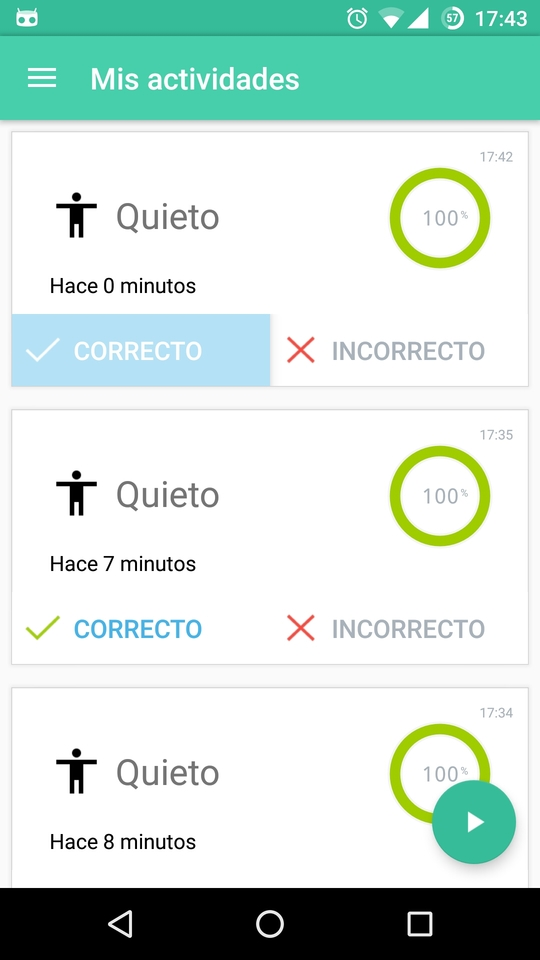
\includegraphics[width=0.33\textwidth]{anexos/graphics/act_ok.jpg}}
 & 
    {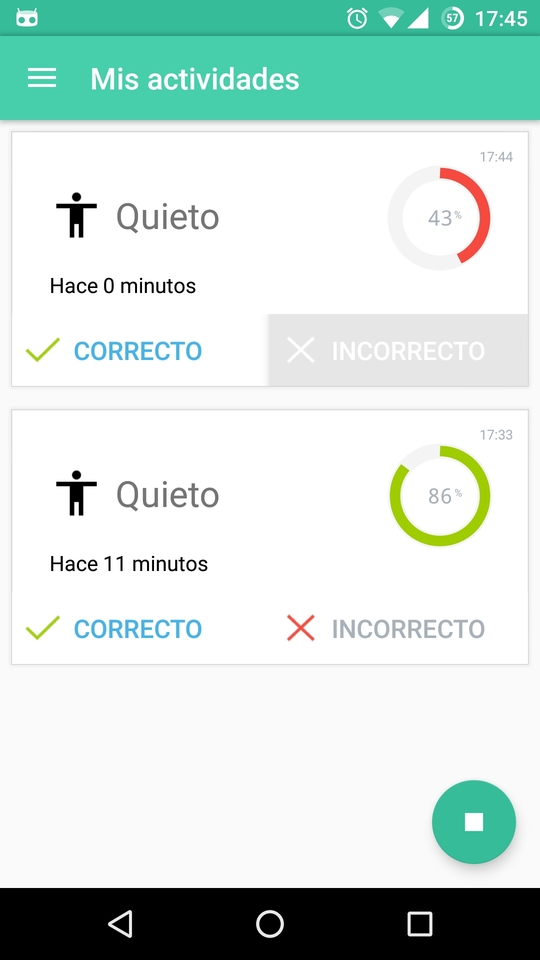
\includegraphics[width=0.33\textwidth]{anexos/graphics/act_nook.jpg}}
 & 
    {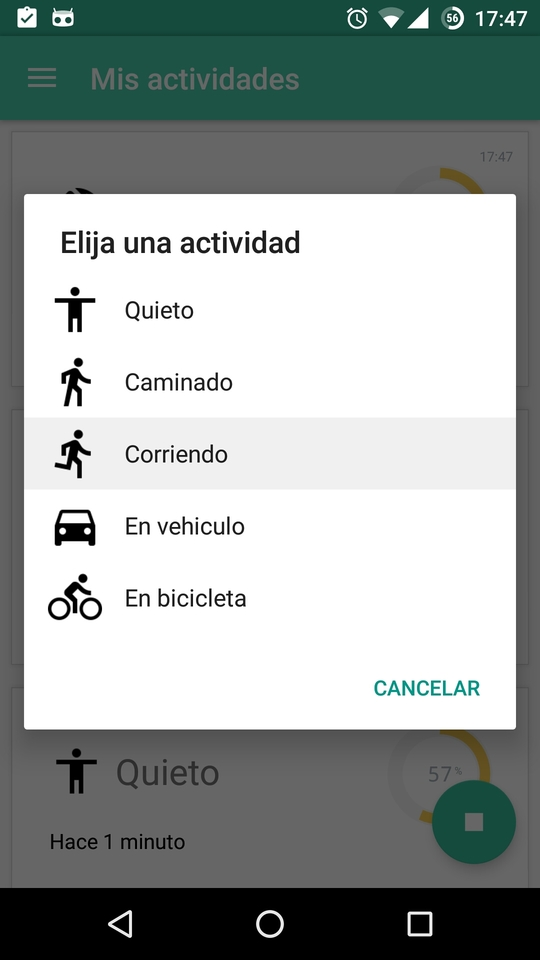
\includegraphics[width=0.33\textwidth]{anexos/graphics/act_feed2.jpg}}
\\
\end{tabular}
    \caption{Responder encuesta de actividades}\label{contrib:actres}
\end{table}

Adicionalmente el servicio puede no detectar ninguna actividad como en la \tabref{contrib:actfeed}.
\begin{quote}
\begin{description}
\item[{Actividad No reconocida}] \leavevmode
El servicio no pudo detectar la activdad física, se debe marcar como incorrecta y proveer la retroalimentación
con la actividad adecuada.

\end{description}
\end{quote}

\begin{table}[!h]
\begin{tabular}{ll}
\textsf{\relax 
Marcar incorrecto (1)
} & \textsf{\relax 
Responder (3)
}\\
    {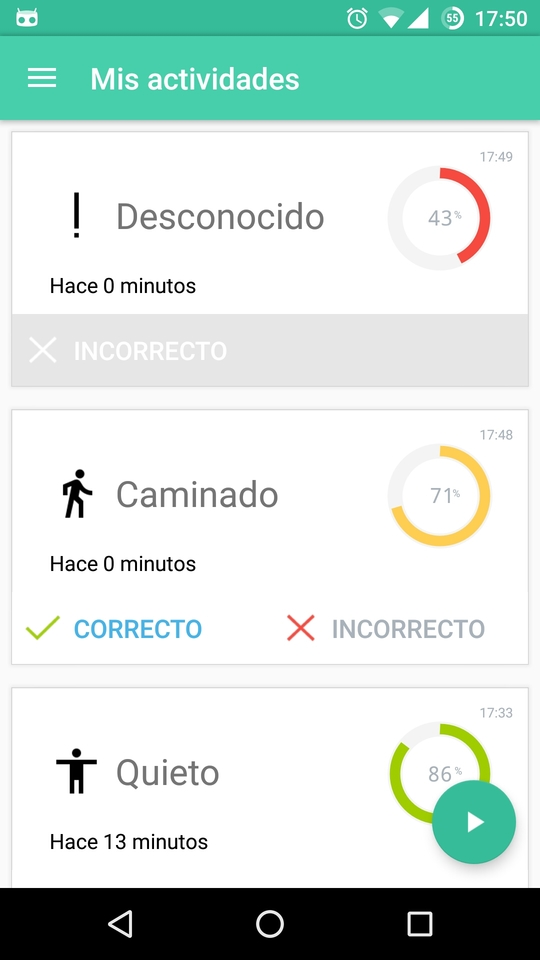
\includegraphics[width=0.33\textwidth]{anexos/graphics/act_nook_unk.jpg}}
 & 
    {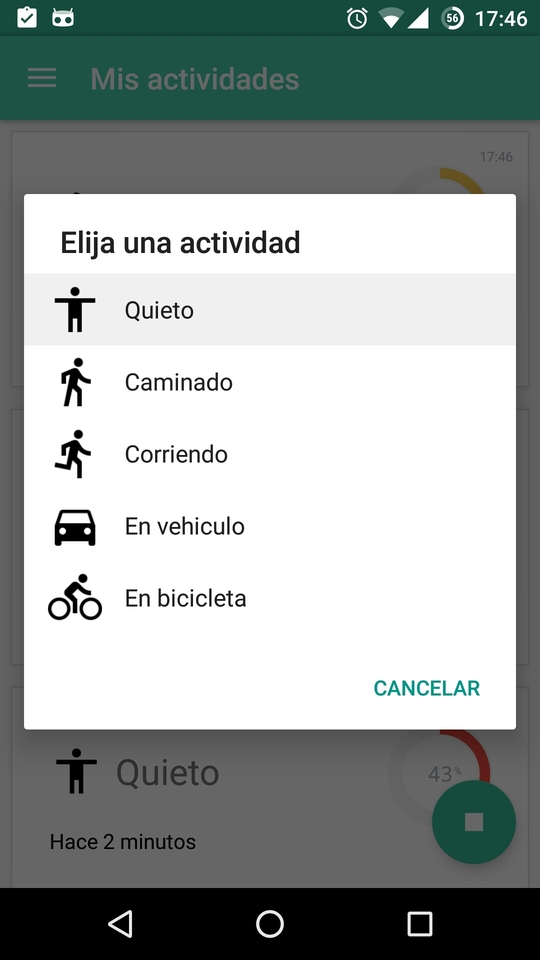
\includegraphics[width=0.33\textwidth]{anexos/graphics/act_feed.jpg}}
\\
\end{tabular}
    \caption{Responder actividad incorrecta con retroalimentación}\label{contrib:actfeed}
\end{table}


\subsection{Configuración Adicional}
\label{config_adic:configuracion-adicional}\label{config_adic:har-conf-advanced}\label{config_adic::doc}

\subsubsection{Activar/Desactivar Servicio}
\label{config_adic:activar-desactivar-servicio}
Desde la barra de menú se puede activar y desactivar el servicio de reconocimiento. Presionar el botón
de acción para elegir ambas opciones como en la \tabref{config_adic:servstart}.

\begin{table}[!h]
\begin{tabular}{lll}
\textsf{\relax 
Desactivar Servicio
} & \textsf{\relax 
Activar el Servicio
} & \textsf{\relax 
Servicio Activado
}\\
    {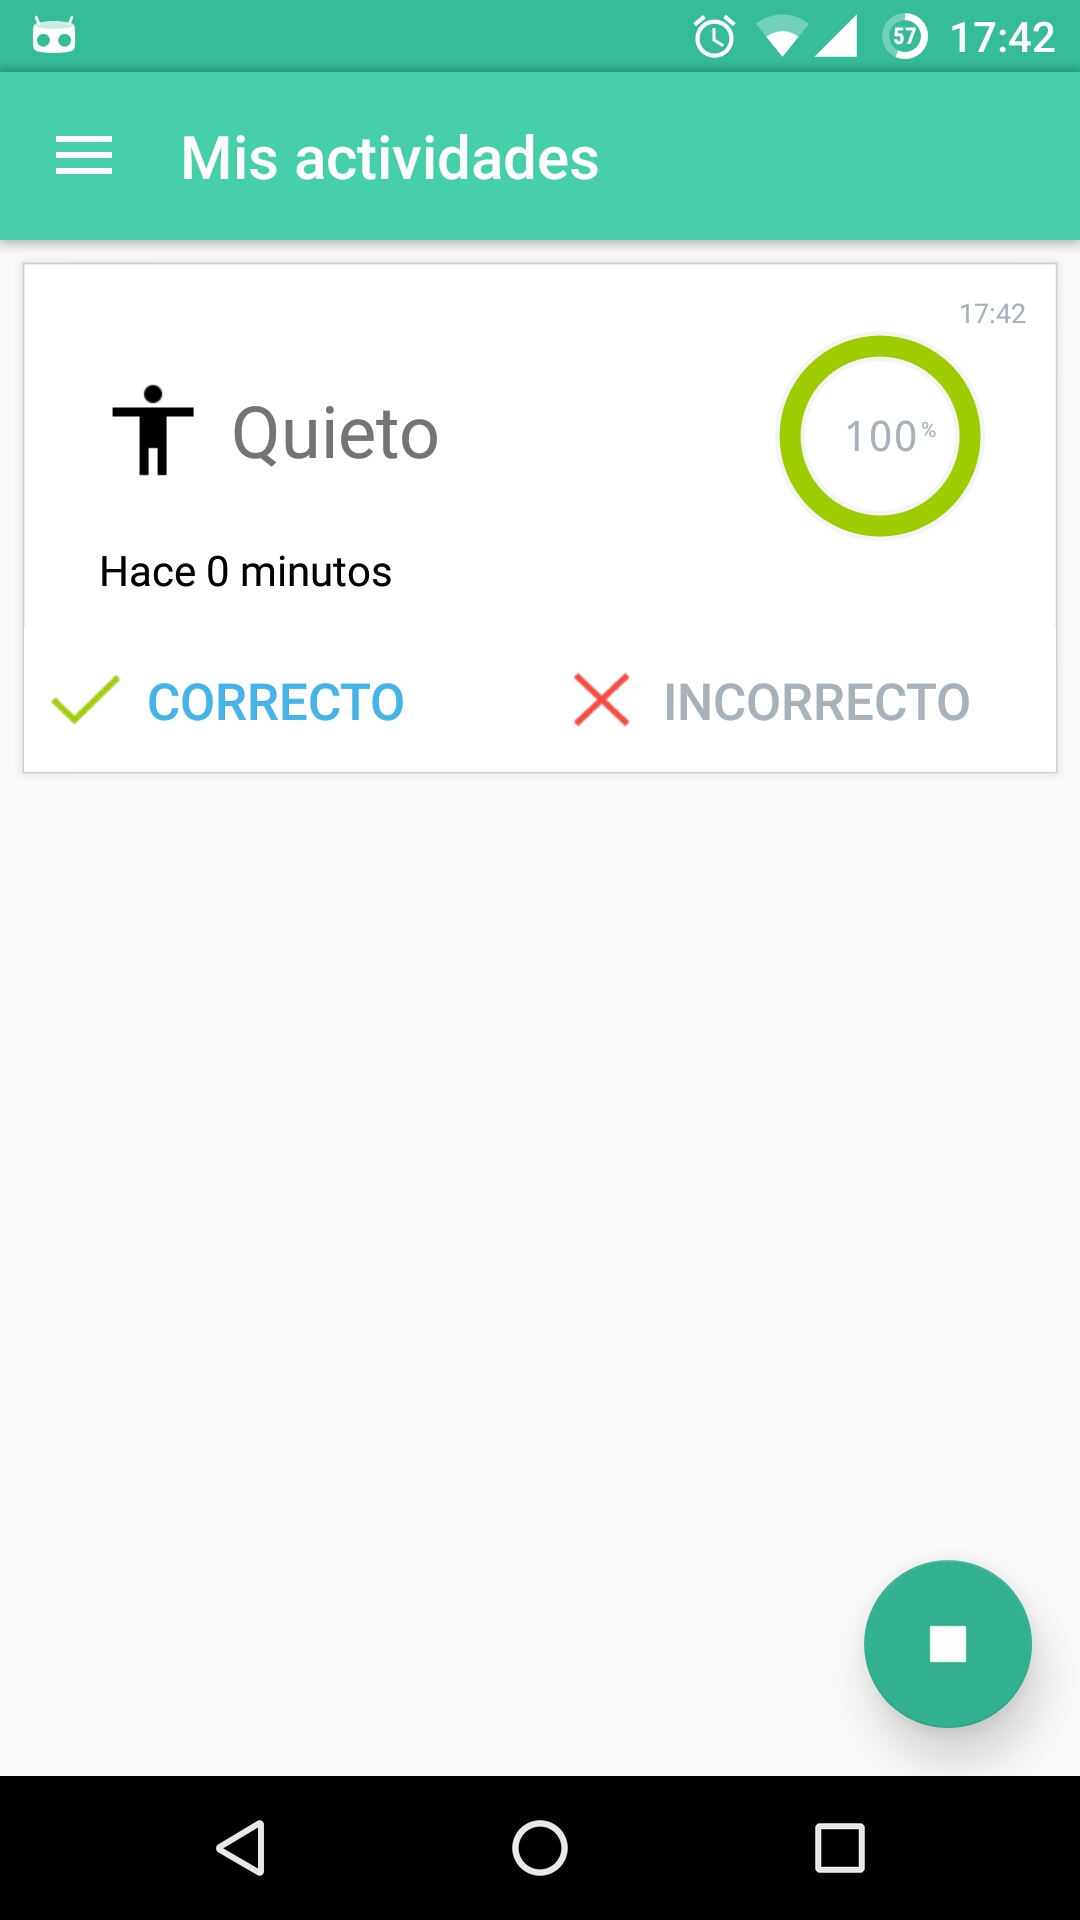
\includegraphics[width=0.33\textwidth]{anexos/graphics/disable_serv.jpg}}
 & 
    {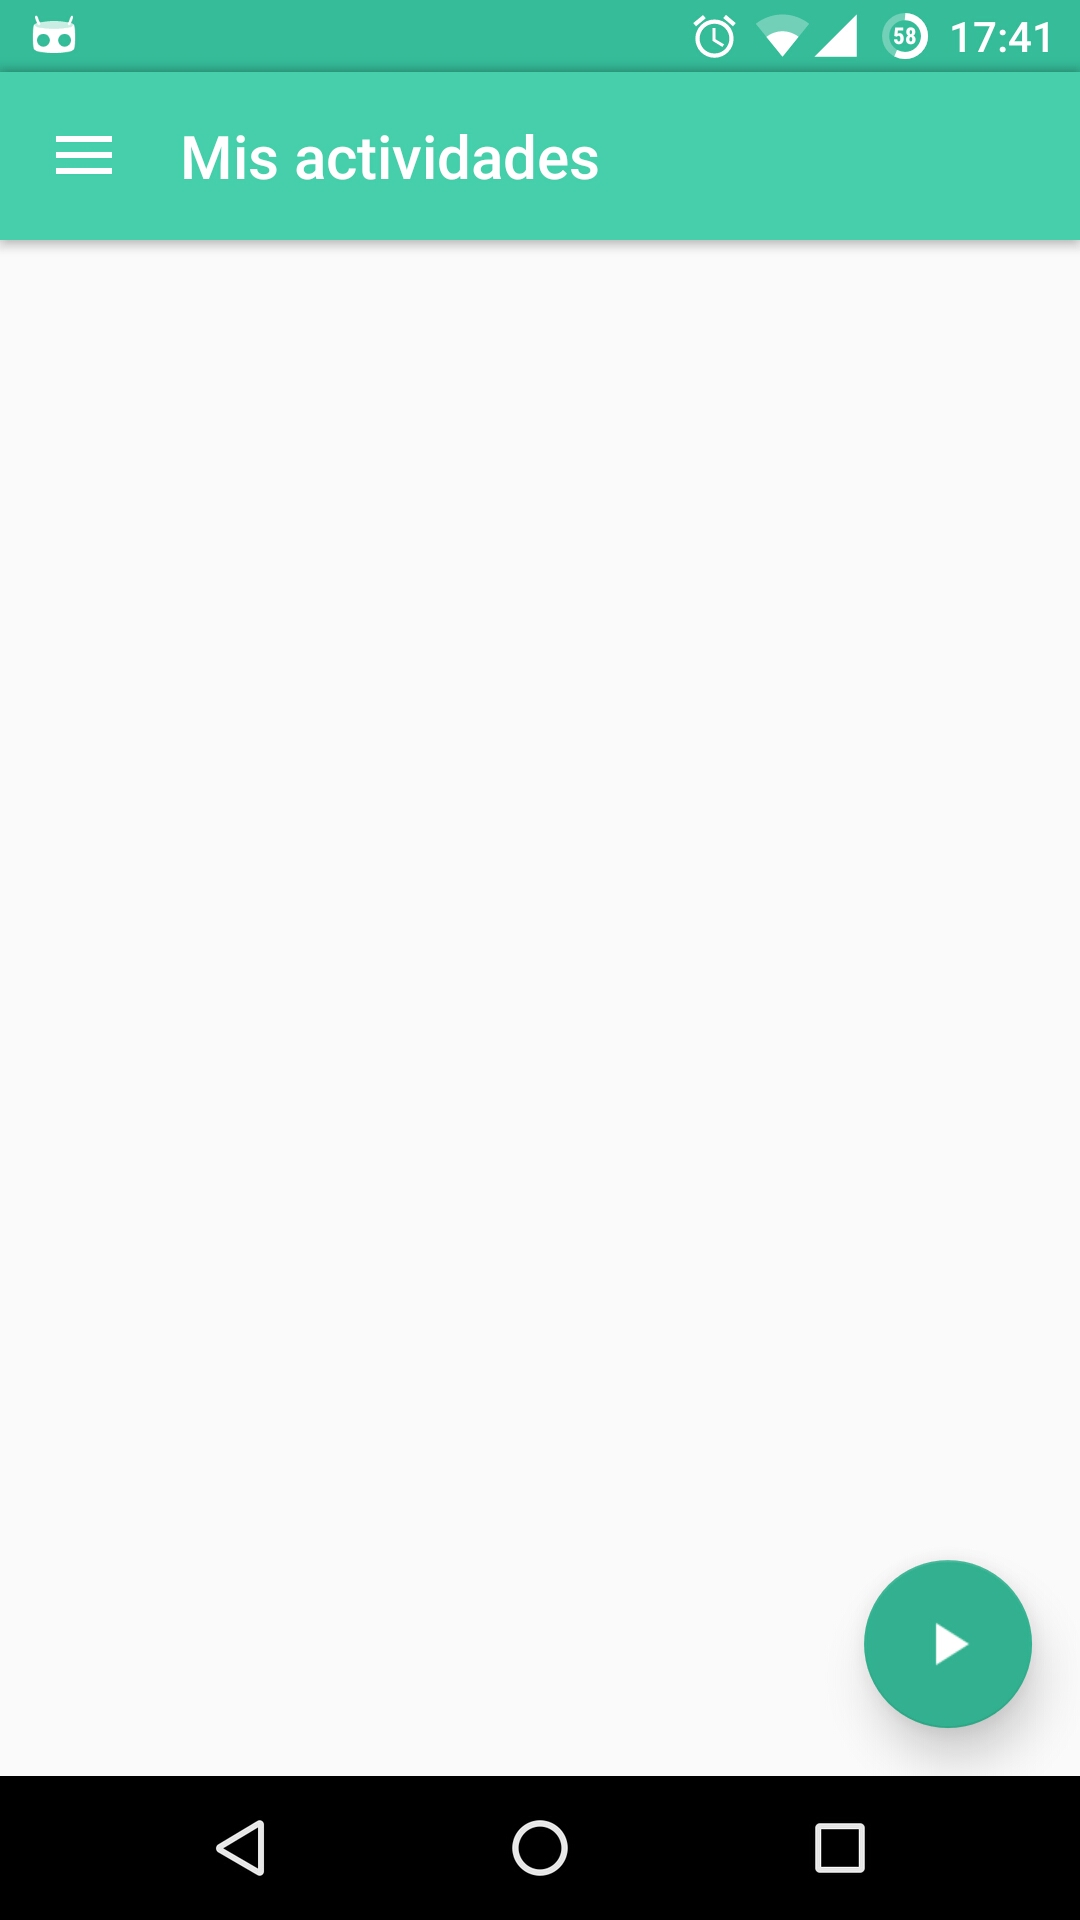
\includegraphics[width=0.33\textwidth]{anexos/graphics/enable_serv.jpg}}
 & 
    {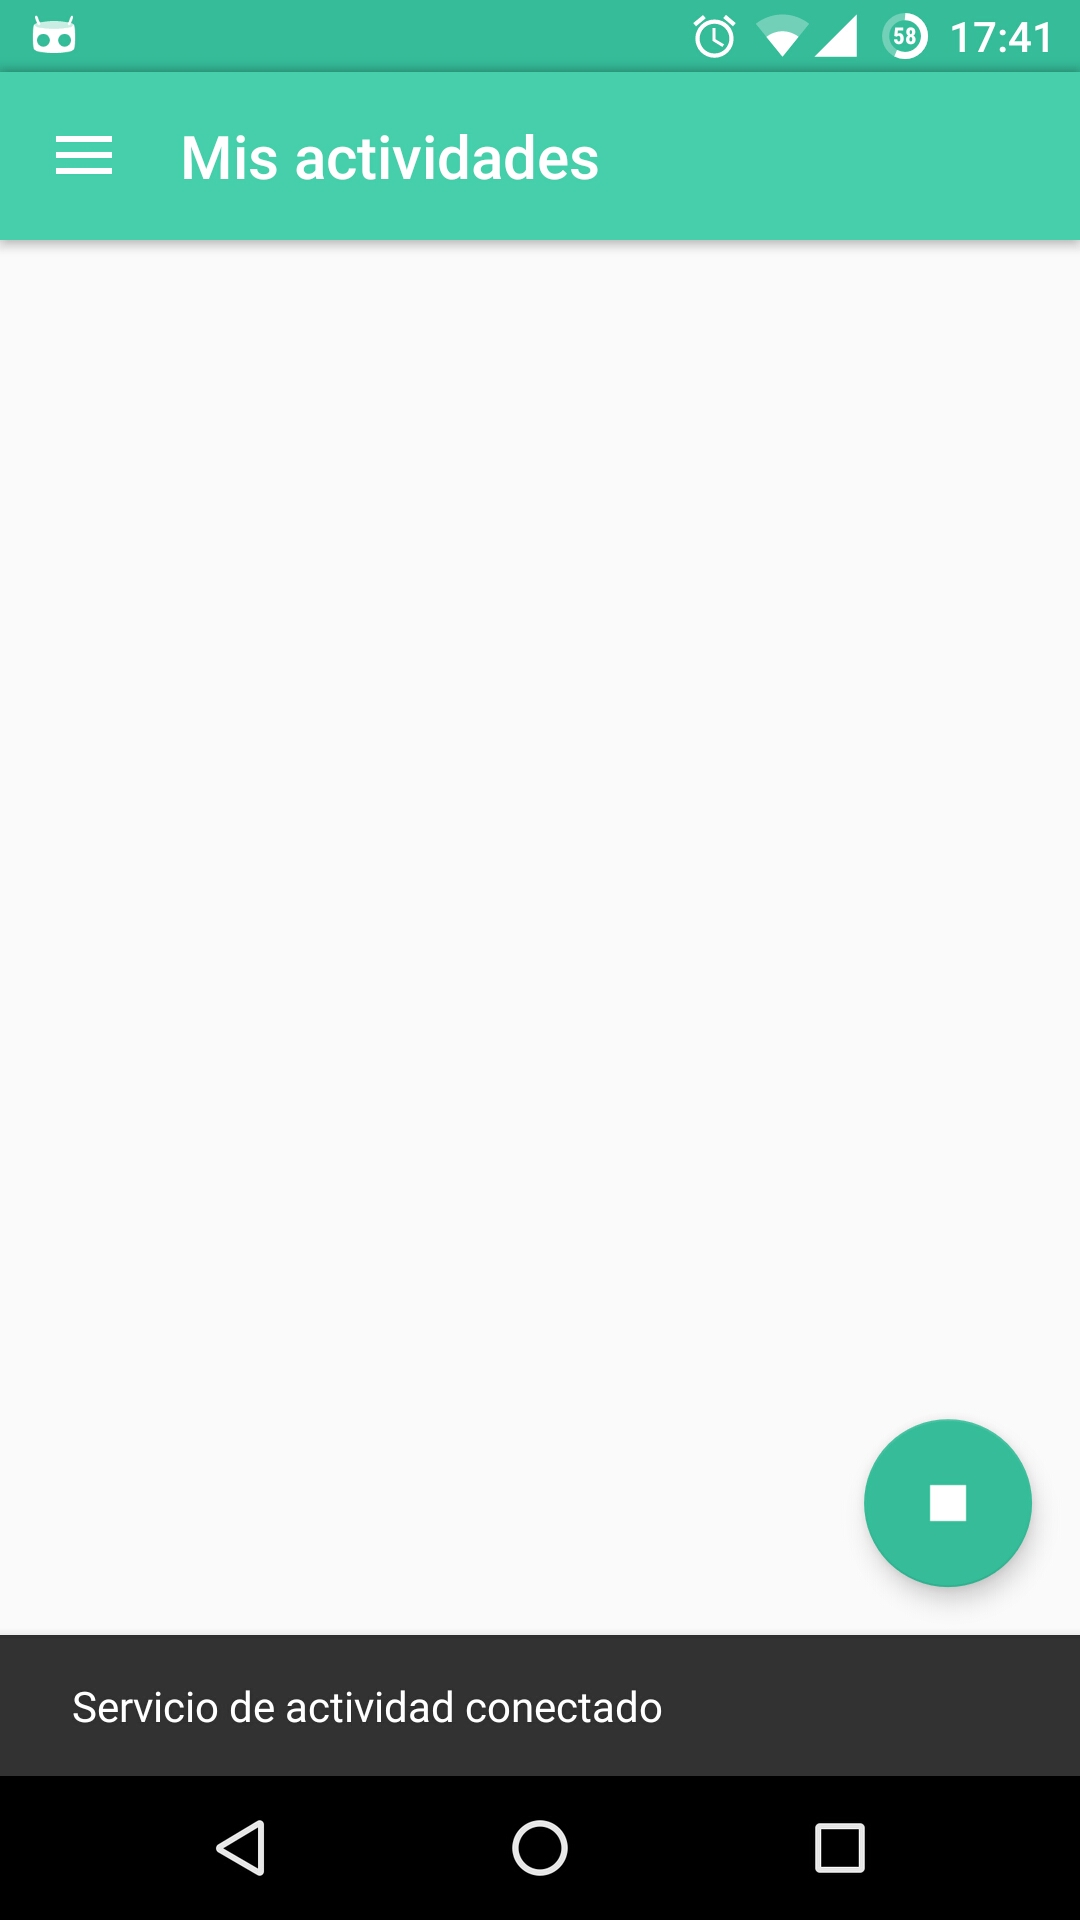
\includegraphics[width=0.33\textwidth]{anexos/graphics/enabled_serv.jpg}}
\\
\end{tabular}
    \caption{Activar y desactivar sesión de reconocimiento}\label{config_adic:servstart}
\end{table}

\subsubsection{Configuración}
\label{config_adic:configuracion}
Para acceder a la configuración desde la aplicación se accede al \code{Menu \textgreater{} Configuración} como en la \figref{config_adic:id1}.
\begin{figure}[!h]
\centering
    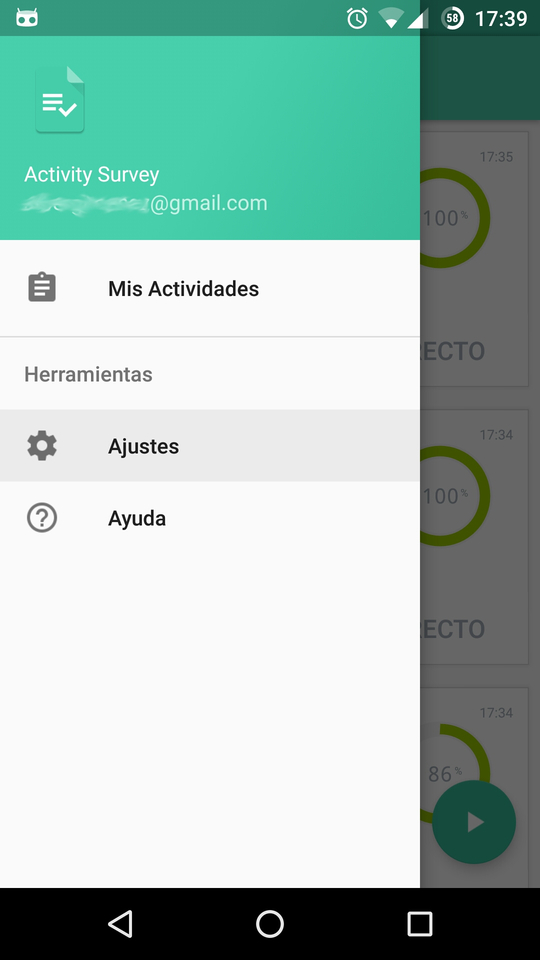
\includegraphics[width=0.4\textwidth]{anexos/graphics/mnu_config.jpg}
\caption{Acceso a la configuración}\label{config_adic:id1}
\end{figure}

En esta vista se  muestra el detalle de los datos enviados al servidor de encuesta y además las opciones
de configuración como en la \figref{config_adic:id2}
\begin{figure}[!h]
    \centering
    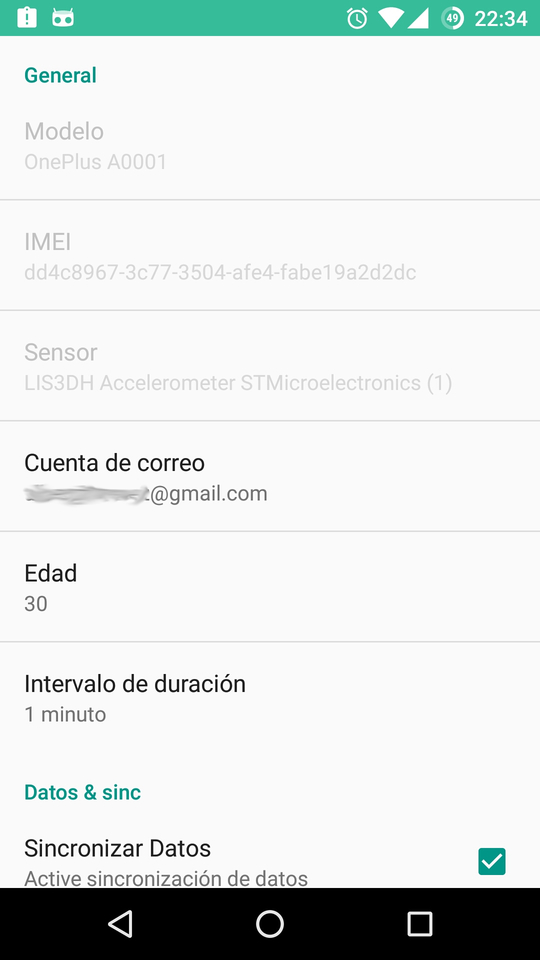
\includegraphics[width=0.4\textwidth]{anexos/graphics/conf_gral.jpg}
\caption{Configuración general}\label{config_adic:id2}
\end{figure}


\paragraph{Correo y Edad}
\label{config_adic:correo-y-edad}
Para cambiar la configuración de correo y edad accede las opciones de la \tabref{config_adic:emedad}.

\begin{table}[!h]
\begin{tabular}{ll}
\textsf{\relax 
Cambiar correo
} & \textsf{\relax 
Cambiar edad
}\\
    {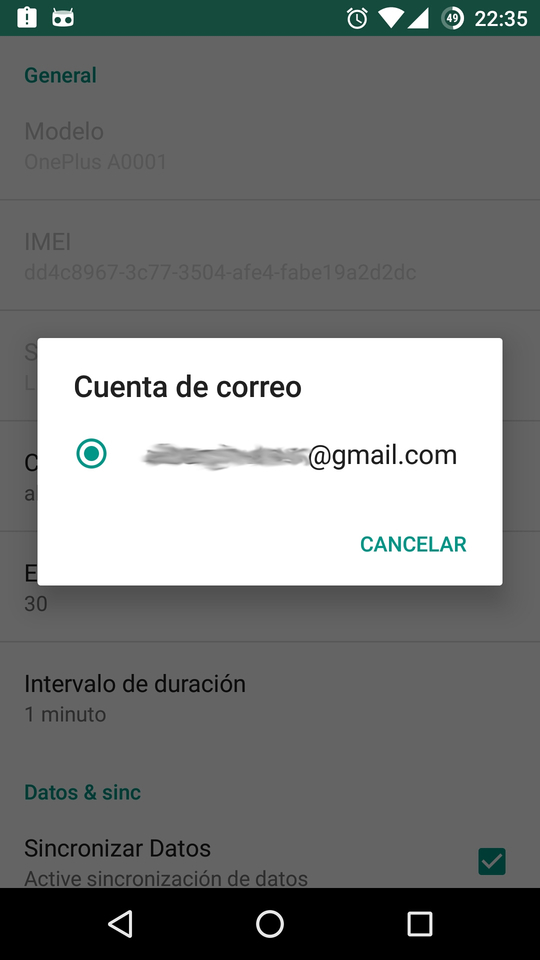
\includegraphics[width=0.33\textwidth]{anexos/graphics/conf_mail.jpg}}
 & 
    {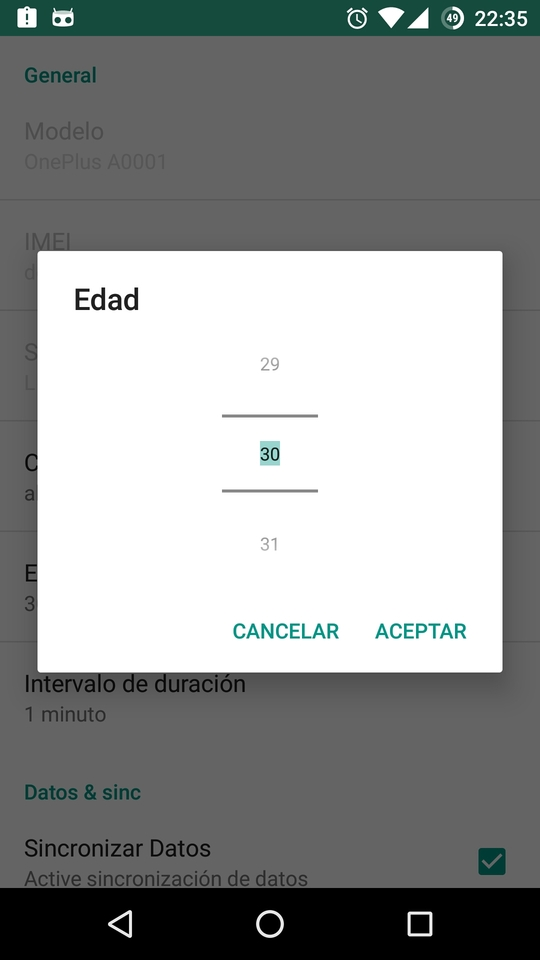
\includegraphics[width=0.33\textwidth]{anexos/graphics/conf_age.jpg}}
\\
\end{tabular}
    \caption{Configuración de correo y edad}\label{config_adic:emedad}
\end{table}

\paragraph{Intervalo}
\label{config_adic:intervalo}
Para cambiar la configuración del intervalo accede a la opción como en la \figref{config_adic:id3}.
\begin{figure}[!h]
    \centering
    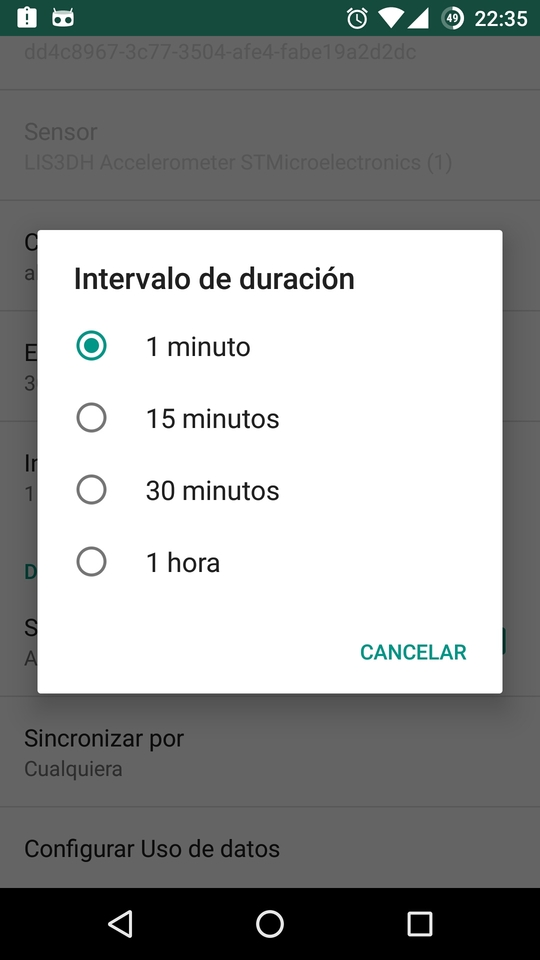
\includegraphics[width=0.4\textwidth]{anexos/graphics/conf_int.jpg}
\caption{Cambiar intervalo}\label{config_adic:id3}
\end{figure}


\paragraph{Sincronización de datos}
\label{config_adic:sincronizacion-de-datos}
Para cambiar la manera en que la aplicación envia los datos por WIFI o redes móviles accede a la opción como en la \tabref{config_adic:conn}.

\begin{table}[!h]
\begin{tabular}{ll}
\textsf{\relax 
Acceso a Sincronizar
} & \textsf{\relax 
Cambiar Sincronizar
}\\
    {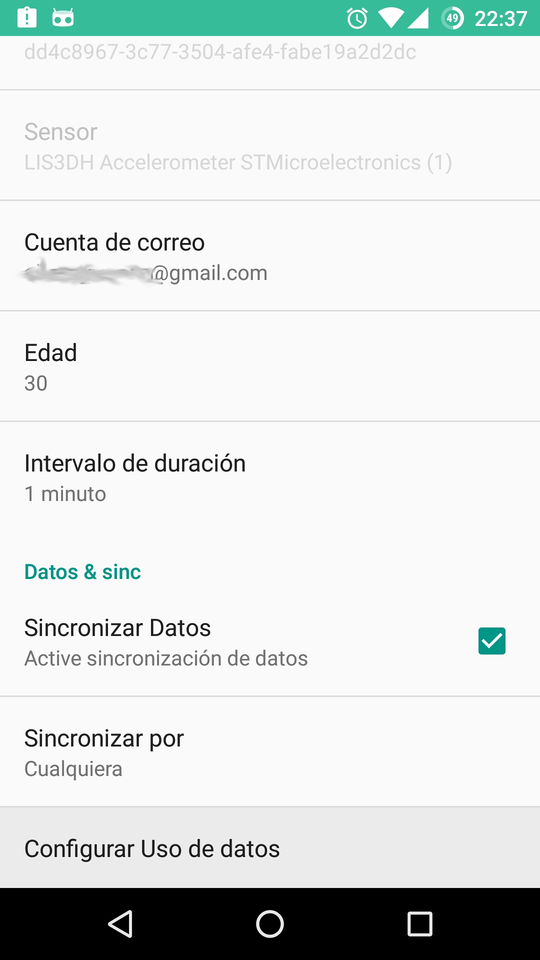
\includegraphics[width=0.33\textwidth]{anexos/graphics/conf_usage.jpg}}
 & 
    {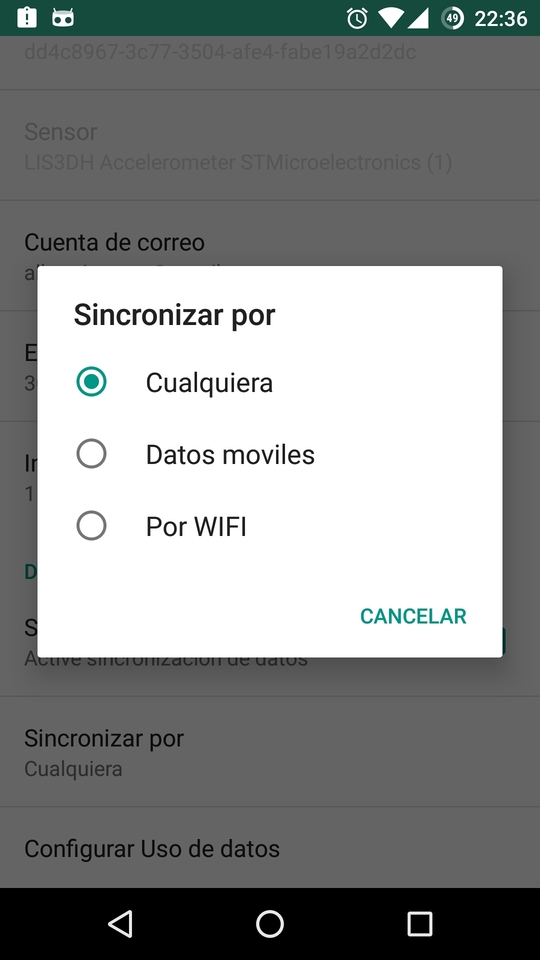
\includegraphics[width=0.33\textwidth]{anexos/graphics/conf_sync.jpg}}
\\
\end{tabular}

\caption{Cambiar preferencias de comunicación}\label{config_adic:conn}
\end{table}

\subsubsection{Ayuda}
\label{config_adic:ayuda}
Para acceder a la guia de ayuda desde la aplicación se accede al \code{Menu \textgreater{} Ayuda} como en la \figref{config_adic:id4}.
\begin{figure}[!h]
    \centering{}
    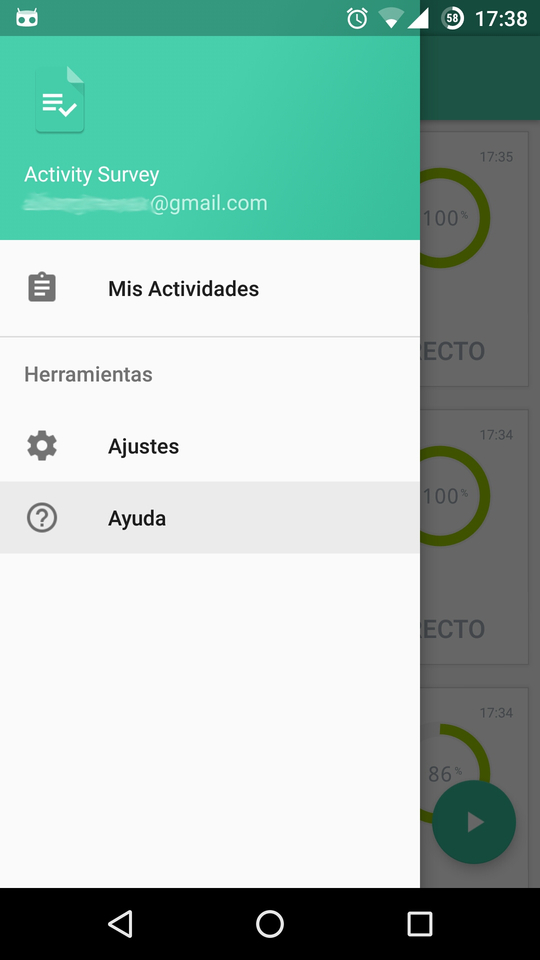
\includegraphics[width=0.4\textwidth]{anexos/graphics/mnu_help.jpg}
\caption{Acceso a la ayuda}\label{config_adic:id4}
\end{figure}

